\documentclass[conference]{IEEEtran}
\IEEEoverridecommandlockouts
% The preceding line is only needed to identify funding in the first footnote. If that is unneeded, please comment it out.
\usepackage{cite}
\usepackage{amsmath,amssymb,amsfonts}
\usepackage{algorithmic}
\usepackage{graphicx}
\usepackage{textcomp}
\usepackage{xcolor}
\usepackage{listings}
\usepackage{float}
\lstset{
basicstyle=\small\ttfamily,
columns=flexible,
breaklines=true
}
\def\BibTeX{{\rm B\kern-.05em{\sc i\kern-.025em b}\kern-.08em
    T\kern-.1667em\lower.7ex\hbox{E}\kern-.125emX}}
\begin{document}

\title{Taichi Based GPU Accelerated Evolutionary Algorithm}

\author{\IEEEauthorblockN{Ali Asghar Chakera}
    \IEEEauthorblockA{\textit{Department of Computer Science} \\
        \textit{Habib University}\\
        Karachi, Pakistan \\
        ay06993@st.habib.edu.pk}
    \and
    \IEEEauthorblockN{Mustafa Sohail}
    \IEEEauthorblockA{\textit{Department of Computer Science} \\
        \textit{Habib University}\\
        Karachi, Pakistan \\
        ms06860@st.habib.edu.pk}
    \and
    \IEEEauthorblockN{Muhammad Mobeen Movania}
    \IEEEauthorblockA{\textit{Department of Computer Science} \\
        \textit{Habib University}\\
        Karachi, Pakistan \\
        mobeen.movania@sse.habib.edu.pk}
}

\maketitle

\begin{abstract}
    Evolutionary algorithms (EAs) have gained significant attention as powerful optimization techniques across various domains due to their ability to efficiently explore solution spaces and find near-optimal solutions. However, the computational demands of EAs, especially for large-scale optimization problems, have prompted the exploration of parallel and GPU-accelerated implementations to enhance their performance. In this paper, we introduce a novel approach leveraging Taichi, a high-performance computing language specifically designed for GPU acceleration, to develop a GPU-accelerated evolutionary algorithm.
\end{abstract}

\begin{IEEEkeywords}
    Taichi, GPU, evolutionary algorithms, optimization
\end{IEEEkeywords}

\section{Introduction}
Evolutionary algorithms (EAs) are a class of computational techniques inspired
by the mechanisms of natural evolution, such as selection, mutation, and
crossover. These algorithms have found widespread application in solving
complex optimization problems, where traditional methods may struggle due to
the complexity and scale of the solution space. The core concept behind EAs is
the iterative generation of candidate solutions, which are evaluated based on a
predefined fitness function. This function assesses the quality or "fitness" of
each solution, guiding the evolutionary process toward optimal or near-optimal
outcomes.

As each iteration requires evaluating the fitness of multiple candidates, the
computational cost can escalate rapidly, especially for problems with high
dimensionality or complex evaluation functions. This computational intensity
can limit the scalability and efficiency of EAs, particularly when applied to
large-scale or time-sensitive optimization tasks. To address this challenge,
parallel computing has emerged as a powerful tool. By distributing the
computational workload across multiple processors or computing nodes, parallel
computing can significantly reduce the time required to execute evolutionary
algorithms.

Recent years have seen an increase in the intersection of evolutionary
algorithms and parallel computing which has opened new avenues for innovation.
This intersectionality has not only accelerated the performance of EAs but also
expanded their applicability to a broader range of optimization challenges,
including real-time applications and large-scale problems.

This paper focuses on the development of a framework for Genetic Algorithms
(GAs) using Taichi, a state-of-the-art programming language designed
specifically for parallel computing. Taichi offers a unique architecture for
high-performance computation which allows developers to write code that can be
efficiently executed across CPUs, GPUs, and other parallel processing units.
The main contribution of this paper is introducing a technique for GPU
accelerated EAs based on Taichi.

The paper is divided into five sections, with section 2 focusing on related
literature, section 3 discussing the methodologies, section 4 highlighting the
results, and section 5 discussing the paper in its entirety.

\section{Literature Review}
The following section will cover the related literature in relation to the
topic of the paper. Literature review is divided in two sections with first
solely focusing on parallelism in GAs, section two discussing work that used
Taichi to optimize EAs in order for a bench-mark to be set.

\subsection{Parallelism in Genetic Algorithms}
GAs are based on natural selection and genetics. They simulate evolution by
iteratively evolving a population of candidate solutions to find the best
outcomes. A GA relies on a population of individuals, or chromosomes, a fitness
function to evaluate them, and operators for selection and mutation.

During a GA's execution, multiple chromosomes are evolved and evaluated
simultaneously, presenting an opportunity to use parallel computing to speed up
the process. With parallel architecture, each chromosome can be generated and
evaluated independently, allowing exploration of the solution space in
parallel. Synchronization is needed only during the selection and crossover
phases, when the entire population is evaluated and knowledge sharing occurs.

According to Hart et al [1], Parallel Genetic Algorithms (PGAs) have the
ability to fend off premature convergence which makes them an ideal solution
technique. This is on top of the fact that PGAs reduce time to locate a
solution and improve the quality of the solution when compared to GAs. The
technique used by Alba et al in [2] uses many elementary GAs performing the
reproductive plan on their own sub-populations. The number of elementary GAs is
another free parameter for Alba et al which they use to their own advantage.

CUDA has been used to solve optimization problems using parallel computing.
Cekmez et al [3] uses nVidia's CUDA Random Number Generation Library (cuRAND)
using GPU's available cores to maximize the parallel throughput. Additionally,
each chromosome is handled in parallel using CUDA. Findings from [3] reported
that the parallel model solved the optimization problem in 1777 times faster
thus highlighting the importance of parallelization. Huang et al [4] aims to
efficiently solve the scheduling problem using the parallelization provided by
CUDA. The results from the paper highlighted that the parallel approach was 19
times faster on 200 jobs for the scheduling algorithm.

Attempts on parallelization of the evolutionary process using CUDA has been
successful in the past when tested on a range of different optimization
problems such as TSP, JSSP, or knapsack.

\subsection{Taichi}
Taichi, developed at the CSAIL lab at the Massachusetts Institute of Technology
(MIT), is a Python-embedded programming language designed for high-performance
parallel computing. It provides significant performance boosts both during
development and at runtime. Taichi has been used in the past for computer
graphics and image segmentation purposes. The original paper on Taichi [5]
highlights how when the performance is compute-bound, our access optimizer can
greatly improve performance by reducing access instruction.

Taichi is particularly well-suited for accelerating Genetic Algorithms (GAs)
due to its emphasis on parallelism and efficiency. It merges the simplicity and
flexibility of Python with the speed and computational power of low-level
parallel programming. One of its key features is its ability to seamlessly
offload computations to GPUs, enabling large-scale parallel processing.

The intuitive integration with Python is a major advantage, as Python is widely
used and familiar to many developers. This seamless integration allows Python
users to harness the power of Taichi without needing to learn a new syntax or
undergo extensive retraining. As a result, developers can quickly prototype and
deploy GA simulations, gaining the benefits of high performance with minimal
additional effort.

However, owing to the fact that Taichi language is relatively new, literature
and work carried out on the language was sparse. To the best of the research
teams capabilities, we were unable to find parallelization techniques of EAs
using Taichi.

\section{Methodology}
The methodology section will cover the implementation details of the
experiment. The section is divided into two parts, the first part will cover
the implementation of the GA using Taichi and the second part will cover the
implementation of the TSP problem.

\subsection{Genetic Algorithm}
The Genetic Algorithm (GA) follows the standard evolutionary process, with the
following components:

\subsubsection{Population Initialization}
The GA starts by initializing a population of candidate solutions. Each
solution is represented as a chromosome, which encodes a potential solution to
the optimization problem. The population size is a configurable parameter that
influences the diversity of the solutions explored.

\subsubsection{Fitness Evaluation}
The fitness of each chromosome is evaluated using a predefined fitness
function. This function assesses the quality of the solution encoded by the
chromosome, guiding the evolutionary process toward optimal or near-optimal
solutions.

\subsubsection{Selection}
A selection mechanism is used to choose parent chromosomes for reproduction
based on their fitness. Higher fitness chromosomes are more likely to be
selected, mimicking the natural selection process. There are various selection
strategies, such as roulette wheel selection, tournament selection, or rank
selection, that can be used to guide the parent selection process. The selected
parent chromosomes are then used to create offspring through crossover and
mutation for the next generation.

\subsubsection{Crossover}
The selected parent chromosomes undergo crossover, where genetic information is
exchanged to create new offspring. This process introduces diversity into the
population, allowing exploration of the solution space.

\subsubsection{Mutation}
To further enhance diversity, mutation is applied to the offspring chromosomes.
This process introduces random changes to the genetic information, preventing
premature convergence and promoting exploration.

\subsubsection{Replacement}
The offspring chromosomes replace the least fit members of the population,
ensuring that the population evolves over time. This process repeats for a
specified number of generations or until a termination condition is met.

\subsection{Traveling Salesman Problem (TSP)}
The Traveling Salesman Problem (TSP) is a classic combinatorial optimization
problem that involves finding the shortest possible route that visits a set of
cities exactly once and returns to the starting city. The objective is to
minimize the total distance traveled. The TSP is a challenging problem due to
its factorial complexity, making it an ideal candidate for testing the efficacy
of evolutionary algorithms. The dataset used for the TSP experiments contains
the coordinates of the cities.

% Show the TSP dataset here
\begin{equation*}
    \textbf{Dataset: } [(x_1, y_1), (x_2, y_2), \dots, (x_n, y_n)]
\end{equation*}

\subsubsection{Problem Representation}
In the context of the TSP, each chromosome represents a potential solution to
the problem. The chromosome encodes the order in which cities are visited,
forming a tour that starts and ends at the same city. The fitness of the
chromosome is determined by the total distance traveled along the tour.
% Show the chromosome representation here
\begin{equation*}
    \textbf{Chromosome: } [1, 2, 3, 4, \dots, n]
\end{equation*}

Here, the numbers represent the index of the cities in the dataset, indicating
the order in which they are visited in the tour.

\subsubsection{Fitness Function}
The fitness function for the TSP evaluates the total distance traveled along
the tour encoded by the chromosome. The distance between each pair of adjacent
cities is calculated using a distance matrix, which contains the distances
between all pairs of cities. The fitness of the chromosome is the sum of the
distances between consecutive cities in the tour.

% Show the fitness function here
\begin{equation*}
    \textbf{Fitness: } f = \sum_{i=1}^{n-1} d(i, i+1) + d(n, 1)
\end{equation*}

Where $d(i, j)$ represents the distance between city $i$ and city $j$ in the
dataset.

\subsubsection{Selection}
The selection process in the TSP GA involves choosing parent chromosomes based
on their fitness. In the context of the TSP, the selection mechanism aims to
favor chromosomes with shorter tour lengths, as they represent better solutions
to the problem. In the experiments, we used truncation selection to choose the
parent chromosomes. Truncation selection selects the top $k$ chromosomes from
the population based on their fitness, where $k$ depends on the offspring
population size.

\subsubsection{Crossover and Mutation}
The crossover and mutation operators for the TSP are designed to preserve the
validity of the tour representation. Crossover involves exchanging genetic
information between parent chromosomes to create offspring, while mutation
introduces random changes to the tour. Both operators are implemented to
maintain the integrity of the tour representation and ensure that the resulting
solutions are valid TSP tours.

In this research, we used point crossover and swap mutation as the genetic
operators for the TSP. Point crossover involves selecting a random point in the
chromosome and exchanging the genetic information beyond that point between the
parent chromosomes.

% Show the point crossover here
\begin{equation*}
    \textbf{Parent 1: } [3, 1, 4, 2, 5]
\end{equation*}
\begin{equation*}
    \textbf{Parent 2: } [5, 2, 1, 4, 3]
\end{equation*}
\begin{equation*}
    \textbf{Offspring 1: } [3, 1, 4, 5, 2]
\end{equation*}
\begin{equation*}
    \textbf{Offspring 2: } [5, 2, 4, 3, 1]
\end{equation*}

To maintain the validity of the tour representation, the offspring chromosomes
are then repaired using a repair operator that ensures that each city is
visited exactly once in the tour. The repair operator loops through the the
parent chromosome until an unvisited city is found and adds it to the
offspring.

Swap mutation involves selecting two random points in the chromosome and
swapping the cities at those points. This introduces random changes to the tour
while maintaining the validity of the solution.

% Show the swap mutation here
\begin{equation*}
    \textbf{Chromosome: } [3, 1, 4, 2, 5]
\end{equation*}
\begin{equation*}
    \textbf{Mutated Chromosome: } [3, 4, 1, 2, 5]
\end{equation*}

The mutation and crossover operators are applied iteratively to the population
of chromosomes, guiding the evolutionary process toward optimal or near-optimal
solutions to the TSP.

\subsection{Implementation using Taichi}
The Genetic Algorithm (GA) for the Traveling Salesman Problem (TSP) was
implemented using Taichi, a high-performance computing language designed for
parallel processing. Since Taichi lang is built on Python, the implementation
required minimal changes to the existing GA code, making it easy to leverage
the power of GPUs for accelerating the evolutionary process. The implementation
consisted of the following steps:

\subsubsection{Population Initialization}
The population of chromosomes was initialized using Taichi's data structures
and parallel computing capabilities. As Taichi leverages GPU for parallel
processing, it requires defining the data structures and operations in a way
that can be efficiently executed on the GPU. Taichi supports 2D arrays which it
converts to linear arrays for GPU processing. The population of chromosomes was
represented as a 2D array, where each row corresponds to a chromosome.

% Show the population initialization code here
\begin{lstlisting}
    population = ti.field(dtype=ti.int32, shape=(population_size, chromosome_size))
    @ti.kernel
    def init_population():
        for i in range(population_size):
            for j in range(chromosome_size):
                population[i, j] = j + 1
            shuffle(i)
            calculate_fitness(i)
\end{lstlisting}

The population was initialized by assigning each chromosome a unique order of
cities and calculating its fitness based on the TSP fitness function. The
shuffle function randomly permutes the order of cities in the chromosome to
introduce diversity in the initial population.

Taichi provides a kernel decorator to define parallel kernels that can be
executed on the GPU. The outer loop in the init\_population kernel is executed
in parallel, with each thread handling a different chromosome in the
population.

\subsubsection{Fitness Evaluation}
Evaluating the fitness of each chromosome in the population is a
computationally intensive task, especially for large populations or complex
fitness functions. However, calculating the fitness of each chromosome can be
parallelized as it involves independent computations for each chromosome. The
fitness function was implemented as a Taichi func that computes the total
distance traveled along the tour encoded by the chromosome on the GPU.

\subsubsection{Selection and Crossover}
The selection and crossover operator was implemented as a Taichi kernel that
selects parent chromosomes based on their fitness. Each pair of parent
chromosomes undergoes crossover to create offspring chromosomes. This process
is parallelized using Taichi's GPU capabilities, with each thread handling a
different pair of parent chromosomes.

The rest of the GA operators, including mutation and replacement remain the
same as the standard GA implementation running sequentially. The
parallelization of the selection and crossover operators significantly
accelerates the evolutionary process, reducing the time required to find
optimal or near-optimal solutions to the TSP.

\section{Experimentation and Results}
\subsection{System Configuration}
The system used for the experiments was a desktop computer with the following
specifications:

\subsubsection{CPU Specifications}
\begin{itemize}
    \item Intel Core i7-9700K @ 3.60GHz
    \item 8 Cores, 8 Threads
    \item 64 GB DDR4 2133 MHz RAM
\end{itemize}

\subsubsection{GPU Specifications}
\begin{itemize}
    \item NVIDIA RTX Titan
    \item 4608 CUDA Cores
    \item 24 GB GDDR6 VRAM
    \item 384-bit Memory Bus
\end{itemize}

\subsection{Experimental Setup}
The experiments were conducted using the qa194 TSP benchmark dataset, which
contains the coordinates of 194 cities in Qatar. The goal was to optimize the
runtime performance of the GA using Taichi and leverage the GPU acceleration to
speed up the evolutionary process.

\subsection{Results}
The results of the experiments demonstrated the effectiveness of the GPU
accelerated GA implemented using Taichi. The runtime performance of the GA was
significantly improved by leveraging the parallel computing capabilities of the
GPU.

The experiments were conducted using different population sizes and
generational counts to evaluate the impact on the runtime performance of the
GA. The results showed that increasing the population size and the number of
generations led to better solutions but also increased the runtime. However,
the GPU acceleration provided by Taichi helped reduce the runtime of the GA,
allowing for faster convergence to optimal or near-optimal solutions.

% Show the runtime comparison graph for different population sizes here
\begin{figure}[H]
    \centerline{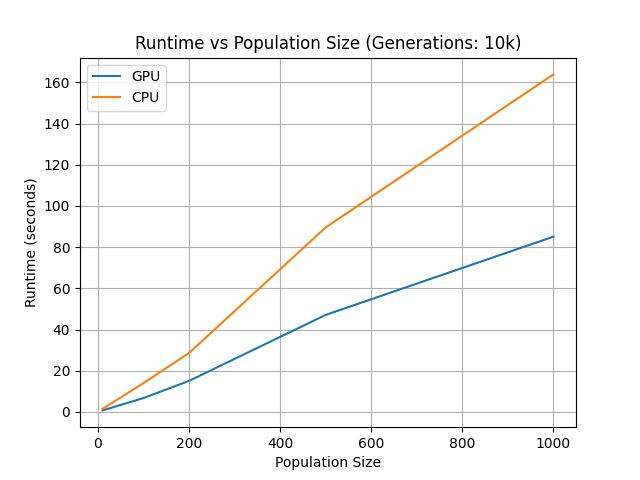
\includegraphics[width=0.5\textwidth]{runtime_vs_population_size.png}}
    \caption{Runtime Comparison for Different Population Sizes}
    \label{fig:1}
\end{figure}

In Figure \ref*{fig:1}, the runtime comparison graph illustrates the runtime
performance of the GPU-accelerated GA and the CPU-based GA for different
population sizes. The results show that the GPU-accelerated GA performed
significantly better than the CPU-based GA, with speedups observed for larger
population sizes.

% Show the runtime comparison graph for different generational counts here
\begin{figure}[H]
    \centerline{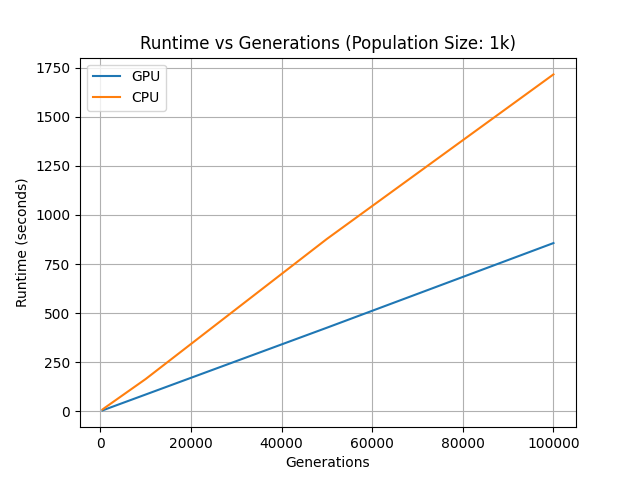
\includegraphics[width=0.5\textwidth]{runtime_vs_generations.png}}
    \caption{Runtime Comparison for Different Generational Counts}
    \label{fig:2}
\end{figure}

Similarly, in Figure \ref*{fig:2}, the runtime comparison graph illustrates the
runtime performance of the GPU-accelerated GA and the CPU-based GA for
different generational counts. The results show that the GPU-accelerated GA was
faster than the CPU-based GA, however, we see that even with the GPU
acceleration, we still see a linear increase in runtime with the increase in
generational counts, this is due to the fact that the genetic operators are
still running sequentially. To further optimize the parallelization of the GA,
we can explore different techniques for parallelizing the genetic operators and
selection strategies such as Island Model.
\section{Future Work and Conclusion}
In this paper, we introduced a novel approach to developing a GPU-accelerated
evolutionary algorithm using Taichi, a high-performance computing language
designed for parallel processing. The experiments conducted on the Traveling
Salesman Problem (TSP) benchmark dataset demonstrated the effectiveness of the
GPU-accelerated GA implemented using Taichi in optimizing the runtime
performance of the evolutionary process.

For future work, we plan to extend the experiments to other optimization
problems and datasets to evaluate the scalability and performance of the
GPU-accelerated GA implemented using Taichi. Additionally, we aim to explore
different genetic operators and selection strategies to further enhance the
efficiency and effectiveness of the evolutionary process. Furthermore, Taichi
provides support for manual thread management which can be used to further
optimize the parallelization of the GA. Moreover, for analysis, the performance
of the GA implemented using Taichi can be compared with other parallel
computing frameworks such as CUDA and PyCUDA to evaluate the relative
performance and efficiency of the GPU-accelerated GA. \section*{Bibliography}

\begin{enumerate}
    \item Hart, W. E., Baden, S., Belew, R. K., \& Kohn, S. (1996, April). Analysis of
          the numerical effects of parallelism on a parallel genetic algorithm. In
          Proceedings of International Conference on Parallel Processing (pp. 606-612).
          IEEE.
    \item Alba, E., \& Troya, J. M. (2002). Improving flexibility and efficiency by
          adding parallelism to genetic algorithms. Statistics and Computing, 12(2),
          91-114.
    \item Cekmez, U., Ozsiginan, M., \& Sahingoz, O. K. (2013, November). Adapting the GA
          approach to solve Traveling Salesman Problems on CUDA architecture. In 2013
          IEEE 14th International Symposium on Computational Intelligence and Informatics
          (CINTI) (pp. 423-428). IEEE.
    \item Huang, C. S., Huang, Y. C., \& Lai, P. J. (2012). Modified genetic algorithms
          for solving fuzzy flow shop scheduling problems and their implementation with
          CUDA. Expert Systems with Applications, 39(5), 4999-5005.
    \item Hu, Y., Li, T. M., Anderson, L., Ragan-Kelley, J., \& Durand, F. (2019).
          Taichi: a language for high-performance computation on spatially sparse data
          structures. ACM Transactions on Graphics (TOG), 38(6), 1-16.
\end{enumerate}

\end{document}
